\graphicspath{{appendices/fig/}}

\chapter{System schematic}
\makeatletter\@mkboth{}{Appendix}\makeatother
\label{appen:system}

\begin{figure}[!h]
    \centering
    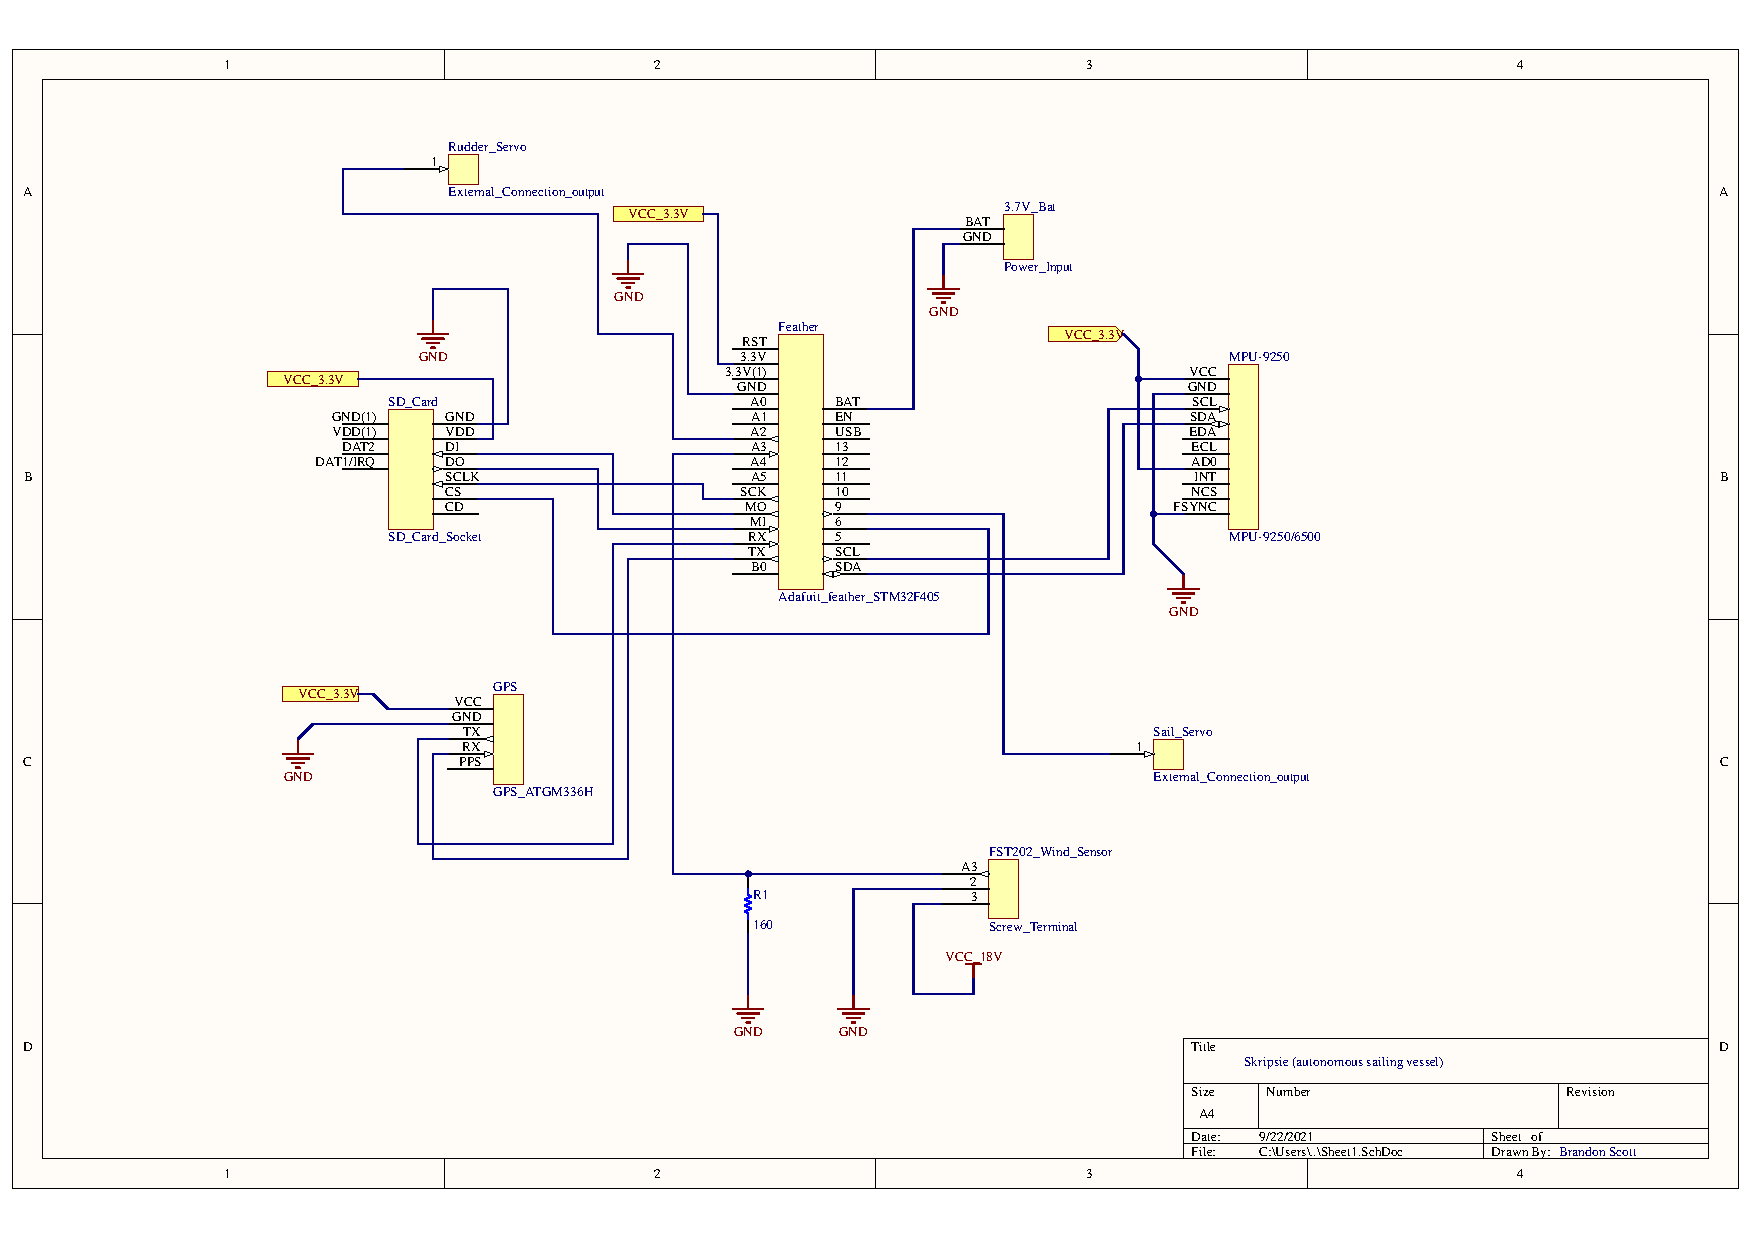
\includegraphics[angle=90,width=0.8\linewidth]{Skripsie-1.pdf}
\end{figure}

\chapter{Software Flow Diagram}
\makeatletter\@mkboth{}{Appendix}\makeatother
\label{appen:flow}

\begin{figure}[!h]
    \centering
    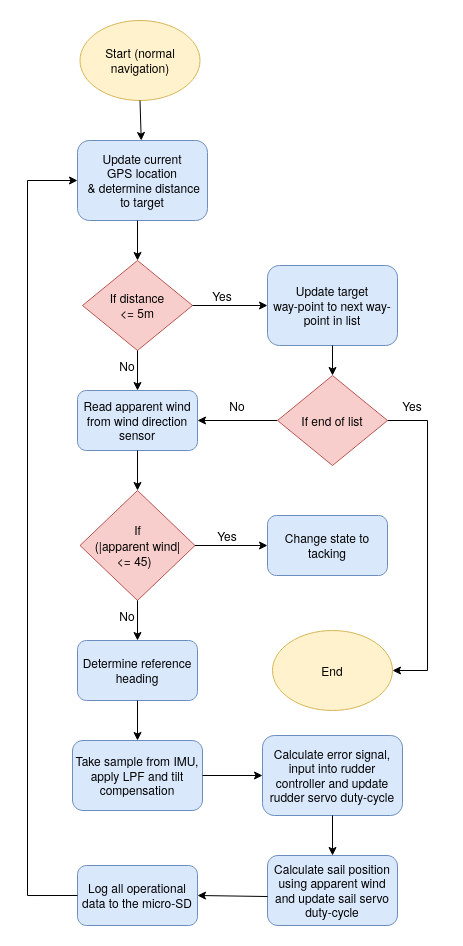
\includegraphics[width=0.5\linewidth]{flow-normal.png}
    \label{fig:normal-flow}
    \caption[Flow diagram of normal navigation state]{Flow diagram of normal navigation state}
\end{figure}

\begin{figure}[!h]
    \centering
    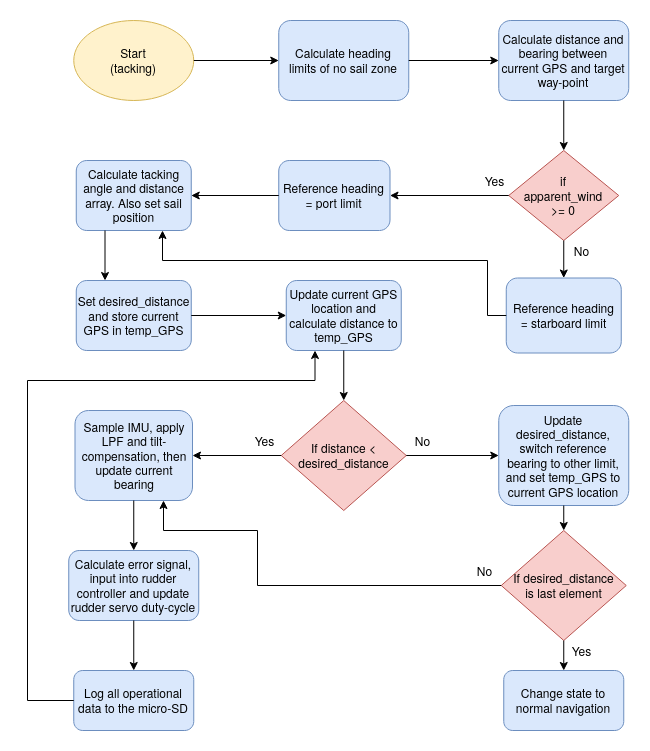
\includegraphics[width=0.7\linewidth]{flow-tacking.png}
    \label{fig:tacking-flow}
    \caption[Flow diagram of tacking state]{Flow diagram of tacking state}
\end{figure}

